% ******************************* PhD Thesis Template **************************
% Please have a look at the README.md file for info on how to use the template

\documentclass[a4paper,12pt,times,numbered,print,index]{Classes/PhDThesisPSnPDF}

% ******************************************************************************
% ******************************* Class Options ********************************
% *********************** See README for more details **************************
% ******************************************************************************

% `a4paper'(The University of Cambridge PhD thesis guidelines recommends a page
% size a4 - default option) or `a5paper': A5 Paper size is also allowed as per
% the Cambridge University Engineering Deparment guidelines for PhD thesis
%
% `11pt' or `12pt'(default): Font Size 10pt is NOT recommended by the University
% guidelines
%
% `oneside' or `twoside'(default): Printing double side (twoside) or single
% side.
%
% `print': Use `print' for print version with appropriate margins and page
% layout. Leaving the options field blank will activate Online version.
%
% `index': For index at the end of the thesis
%
% `draft': For draft mode without loading any images (same as draft in book)
%
% `draftmode': Special draft mode with line numbers, images, and water mark with
% timestamp and custom text. Position of the text can also be modified.
%
% `abstract': To generate only the title page and abstract page with
% dissertation title and name, to submit to the Student Registry
%
% `chapter`: This option enables only the specified chapter and it's references
%  Useful for review and corrections.
%
% ************************* Custom Page Margins ********************************
%
% `custommargin`: Use `custommargin' in options to activate custom page margins,
% which can be defined in the preamble.tex. Custom margin will override
% print/online margin setup.
%
% *********************** Choosing the Fonts in Class Options ******************
%
% `times' : Times font with math support. (The Cambridge University guidelines
% recommend using times)
%
% `fourier': Utopia Font with Fourier Math font (Font has to be installed)
%            It's a free font.
%
% `customfont': Use `customfont' option in the document class and load the
% package in the preamble.tex
%
% default or leave empty: `Latin Modern' font will be loaded.
%
% ********************** Choosing the Bibliography style ***********************
%
% `authoryear': For author-year citation eg., Krishna (2013)
%
% `numbered': (Default Option) For numbered and sorted citation e.g., [1,5,2]
%
% `custombib': Define your own bibliography style in the `preamble.tex' file.
%              `\RequirePackage[square, sort, numbers, authoryear]{natbib}'.
%              This can be also used to load biblatex instead of natbib
%              (See Preamble)
%
% **************************** Choosing the Page Style *************************
%
% `default (leave empty)': For Page Numbers in Header (Left Even, Right Odd) and
% Chapter Name in Header (Right Even) and Section Name (Left Odd). Blank Footer.
%
% `PageStyleI': Chapter Name next & Page Number on Even Side (Left Even).
% Section Name & Page Number in Header on Odd Side (Right Odd). Footer is empty.
%
% `PageStyleII': Chapter Name on Even Side (Left Even) in Header. Section Number
% and Section Name in Header on Odd Side (Right Odd). Page numbering in footer


% ********************************** Preamble **********************************
% Preamble: Contains packages and user-defined commands and settings
% ******************************************************************************
% ****************************** Custom Margin *********************************

% Add `custommargin' in the document class options to use this section
% Set {innerside margin / outerside margin / topmargin / bottom margin}  and
% other page dimensions
\ifsetCustomMargin
  \RequirePackage[left=37mm,right=30mm,top=35mm,bottom=30mm]{geometry}
  \setFancyHdr % To apply fancy header after geometry package is loaded
\fi

% *****************************************************************************
% ******************* Fonts (like different typewriter fonts etc.)*************

% Add `customfont' in the document class option to use this section

\ifsetCustomFont
  % Set your custom font here and use `customfont' in options. Leave empty to
  % load computer modern font (default LaTeX font).
  \RequirePackage{helvet}
\fi

% *****************************************************************************
% **************************** Custom Packages ********************************

% ************************* Algorithms and Pseudocode **************************

%\usepackage{algpseudocode}


% ********************Captions and Hyperreferencing / URL **********************

% Captions: This makes captions of figures use a boldfaced small font.
%\RequirePackage[small,bf]{caption}

\RequirePackage[labelsep=space,tableposition=top]{caption}
\renewcommand{\figurename}{Fig.} %to support older versions of captions.sty


% *************************** Graphics and figures *****************************

%\usepackage{rotating}
%\usepackage{wrapfig}

% Uncomment the following two lines to force Latex to place the figure.
% Use [H] when including graphics. Note 'H' instead of 'h'
%\usepackage{float}
%\restylefloat{figure}

% Subcaption package is also available in the sty folder you can use that by
% uncommenting the following line
% This is for people stuck with older versions of texlive
%\usepackage{sty/caption/subcaption}
\usepackage{subcaption}

% ********************************** Tables ************************************
\usepackage{booktabs} % For professional looking tables
\usepackage{multirow}

%\usepackage{multicol}
%\usepackage{longtable}
%\usepackage{tabularx}


% ***************************** Math and SI Units ******************************

\usepackage{amsfonts}
\usepackage{amsmath}
\usepackage{amssymb}
\usepackage{siunitx} % use this package module for SI units


% ******************************* Line Spacing *********************************

% Choose linespacing as appropriate. Default is one-half line spacing as per the
% University guidelines

% \doublespacing
% \onehalfspacing
% \singlespacing


% ************************ Formatting / Footnote *******************************

% Don't break enumeration (etc.) across pages in an ugly manner (default 10000)
%\clubpenalty=500
%\widowpenalty=500

%\usepackage[perpage]{footmisc} %Range of footnote options


% *****************************************************************************
% *************************** Bibliography  and References ********************

%\usepackage{cleveref} %Referencing without need to explicitly state fig /table

% Add `custombib' in the document class option to use this section
\ifuseCustomBib
   \RequirePackage[square, sort, numbers, authoryear]{natbib} % CustomBib

% If you would like to use biblatex for your reference management, as opposed to the default `natbibpackage` pass the option `custombib` in the document class. Comment out the previous line to make sure you don't load the natbib package. Uncomment the following lines and specify the location of references.bib file

%\RequirePackage[backend=biber, style=numeric-comp, citestyle=numeric, sorting=nty, natbib=true]{biblatex}
%\bibliography{References/references} %Location of references.bib only for biblatex

\fi

% changes the default name `Bibliography` -> `References'
\renewcommand{\bibname}{References}


% *****************************************************************************
% *************** Changing the Visual Style of Chapter Headings ***************
% This section on visual style is from https://github.com/cambridge/thesis

% Uncomment the section below. Requires titlesec package.

%\RequirePackage{titlesec}
%\newcommand{\PreContentTitleFormat}{\titleformat{\chapter}[display]{\scshape\Large}
%{\Large\filleft{\chaptertitlename} \Huge\thechapter}
%{1ex}{}
%[\vspace{1ex}\titlerule]}
%\newcommand{\ContentTitleFormat}{\titleformat{\chapter}[display]{\scshape\huge}
%{\Large\filleft{\chaptertitlename} \Huge\thechapter}{1ex}
%{\titlerule\vspace{1ex}\filright}
%[\vspace{1ex}\titlerule]}
%\newcommand{\PostContentTitleFormat}{\PreContentTitleFormat}
%\PreContentTitleFormat


% ******************************************************************************
% ************************* User Defined Commands ******************************
% ******************************************************************************

% *********** To change the name of Table of Contents / LOF and LOT ************

%\renewcommand{\contentsname}{My Table of Contents}
%\renewcommand{\listfigurename}{My List of Figures}
%\renewcommand{\listtablename}{My List of Tables}


% ********************** TOC depth and numbering depth *************************

\setcounter{secnumdepth}{2}
\setcounter{tocdepth}{2}


% ******************************* Nomenclature *********************************

% To change the name of the Nomenclature section, uncomment the following line

%\renewcommand{\nomname}{Symbols}


% ********************************* Appendix ***********************************

% The default value of both \appendixtocname and \appendixpagename is `Appendices'. These names can all be changed via:

%\renewcommand{\appendixtocname}{List of appendices}
%\renewcommand{\appendixname}{Appndx}

% ******************************** Draft Mode **********************************

% Uncomment to disable figures in `draftmode'
%\setkeys{Gin}{draft=true}  % set draft to false to enable figures in `draft'

% These options are active only during the draft mode
% Default text is "Draft"
%\SetDraftText{DRAFT}

% Default Watermark location is top. Location (top/bottom)
%\SetDraftWMPosition{bottom}

% Draft Version - default is v1.0
%\SetDraftVersion{v1.1}

% Draft Text grayscale value (should be between 0-black and 1-white)
% Default value is 0.75
%\SetDraftGrayScale{0.8}


%% Todo notes functionality
%% Uncomment the following lines to have todonotes.

%\ifsetDraft
%	\usepackage[colorinlistoftodos]{todonotes}
%	\newcommand{\mynote}[1]{\todo[author=kks32,size=\small,inline,color=green!40]{#1}}
%\else
%	\newcommand{\mynote}[1]{}
%	\newcommand{\listoftodos}{}
%\fi

% Example todo: \mynote{Hey! I have a note}




% ************************ Thesis Information & Meta-data **********************
% Thesis title and author information, refernce file for biblatex
% ************************ Thesis Information & Meta-data **********************
%% The title of the thesis
\title{Writing your PhD thesis in \texorpdfstring{\\ \LaTeX2e}{LaTeX2e}}
%\texorpdfstring is used for PDF metadata. Usage:
%\texorpdfstring{LaTeX_Version}{PDF Version (non-latex)} eg.,
%\texorpdfstring{$sigma$}{sigma}

%% Subtitle (Optional)
\subtitle{Using the CUED template}

%% The full name of the author
\author{Krishna Kumar}

%% Department (eg. Department of Engineering, Maths, Physics)
\dept{Department of Engineering}

%% University and Crest
\university{University of Cambridge}
\crest{
\includegraphics[width=0.25\textwidth]{University_Crest}}

%% You can redefine the submission text:
% Default as per the University guidelines:
% ``This dissertation is submitted for the degree of''
%\renewcommand{\submissiontext}{change the default text here if needed}

%% Full title of the Degree
\degree{Doctor of Philosophy}

%% College affiliation (optional)
\college{King's College}

%% Submission date
% Default is set as {\monthname[\the\month]\space\the\year}
%\degreedate{September 2014} 

%% Meta information
\subject{LaTeX} \keywords{{LaTeX} {PhD Thesis} {Engineering} {University of
Cambridge}}


% ***************************** Abstract Separate ******************************
% To printout only the titlepage and the abstract with the PhD title and the
% author name for submission to the Student Registry, use the `abstract' option in
% the document class.

\ifdefineAbstract
 \pagestyle{empty}
 \includeonly{Declaration/declaration, Abstract/abstract}
\fi

% ***************************** Chapter Mode ***********************************
% The chapter mode allows user to only print particular chapters with references
% Title, Contents, Frontmatter are disabled by default
% Useful option to review a particular chapter or to send it to supervisior.
% To use choose `chapter' option in the document class

\ifdefineChapter
 \includeonly{Chapter3/chapter3}
\fi

% ******************************** Front Matter ********************************
\begin{document}

\frontmatter

\begin{titlepage}
  \maketitle
\end{titlepage}


% ******************************* Thesis Dedidcation ********************************

\begin{dedication} 

I would like to dedicate this report to my school teachers who said I was too lazy to amount to anything. 

\end{dedication}


% ******************************* Thesis Declaration ********************************

\begin{declaration}

I hereby declare that except where specific reference is made to the work of others, the contents of this dissertation are original and have not been submitted in whole or in part for consideration for any other degree or qualification in this, or any other University. This dissertation is the result of my own work and includes nothing which is the outcome of work done in collaboration, except where specifically indicated in the text. This dissertation contains less than 65,000 words including appendices, bibliography, footnotes, tables and equations and has less than 150 figures.

% Author and date will be inserted automatically from thesis.tex \author \degreedate

\end{declaration}


% ************************** Thesis Acknowledgements *****************************

\begin{acknowledgements}      


And I would like to acknowledge firstly Dr. Andrew Pomfret %TODO  


\end{acknowledgements}

% ************************** Thesis Abstract *****************************
% Use `abstract' as an option in the document class to print only the titlepage and the abstract.
\begin{abstract}
This is where you write your abstract ...
\end{abstract}


% *********************** Adding TOC and List of Figures ***********************

\tableofcontents

\listoffigures

\listoftables

% \printnomencl[space] space can be set as 2em between symbol and description
%\printnomencl[3em]

\printnomencl

% ******************************** Main Matter *********************************
\mainmatter

%******************************************************************************************************
%*********************************** First Chapter ****************************************************
%******************************************************************************************************

\chapter{Introduction}  %Title of the First Chapter
\label{intro}

% **************************** Define Graphics Path **************************
\ifpdf
    \graphicspath{{Chapter1/Figs/Raster/}{Chapter1/Figs/PDF/}{Chapter1/Figs/}}
\else
    \graphicspath{{Chapter1/Figs/Vector/}{Chapter1/Figs/}}
\fi


%******************************************************************************************************
%******************************************************************************************************
\section{An Introduction to Unmanned Aerial Vehicles} 
\label{intro:UAVs}

The term Unmanned Aerial Vehicle (UAV) can be used to describe any form of aircraft that does not require a pilot on board. This term includes aircraft that are controlled remotely, autonomous vehicles capable of navigating themselves, and any aircraft that are a combination of the two. Other terms that may be familiar are ``drone'' and Unmanned Aerial System (UAS), which can be used interchangeably with UAV within the context of this project. 

UAVs come in a wide range of form factors but can be split into two main classes; fixed-wing UAVs and rotary wing UAVs. Fixed-wing UAVs are generally only capable of horizontal take-off and landing (HTOL), whilst rotary wing UAVs generally employ vertical take-off and landing (VTOL). There are, however, other forms of UAV which incorporate features of both main classes; for example, quadplane UAVS use rotary wing rotors to allow VTOL, but do the main bulk of their flying with forward facing rotors much like a fixed-wing UAV. Across these categories are a very wide range of UAV platforms, from hobbyist quadcopters to military attack vehicles, and many many others in between. %TODO images?  
Although the range of UAV form factors and their uses is vast, the vast majority are suitable for candidates for complete autonomous flight control, as shall be described in Section %TODO reference where we talk about adding hardware modules 
 
Although there were a large number of suitable candidates for the following work, it was decided that this project would be aimed at the control of strictly fixed-wing UAVs for the purposes of aerial photography. For that reason, we shall not discuss any other style of UAV. %TODO 

%******************************************************************************************************
%******************************************************************************************************
\section{UAVs for Aerial Photography} 
\label{intro:photography}

The first recorded use of aerial photography was in 1858 by a French balloonist and photographer known as ``Nadar'' at a height of 80 metres using a tethered hot air balloon. %TODO ref aerial photography history
Since then aerial photography has of course massively progressed, both in terms of the aerial vehicles in use and the cameras available. As such, it is now an activity that can be partaken in by both organisations, companies, and individuals alike, for a range of purposes. For example, aerial photography of course plays a very large role in intelligence gathering by government agencies and militaries, but can also be a hobby for otherwise earth-bound photography enthusiasts. 

Different applications will require different equipment and styles of photography; a hobbyist may want a wide panorama, whilst a mapping application will require a consistent vertical camera angle. The use of aerial photography for mapping or measurement is known as aerial photogrammetry, and will be the chosen field of interest for this project. Aerial photogrammetry is a specific subset of aerial photography in that it not only requires the capturing of images, but additional information about how and where the image was captured. For this project, we are looking at the use of aerial photogrammetry to create an image of the land below our UAV. In order to be able to do this, we need to be able to capture a set of images, and know the location of the UAV when the images were captured, to allow the images to be stitched together into one larger image of the ground beneath. In this scenario we can typically use GPS co-ordinates and a pre-planned imaging path to define which images relate to which areas of the ground below. %TODO more






\begin{figure}[htbp!] 
\centering    
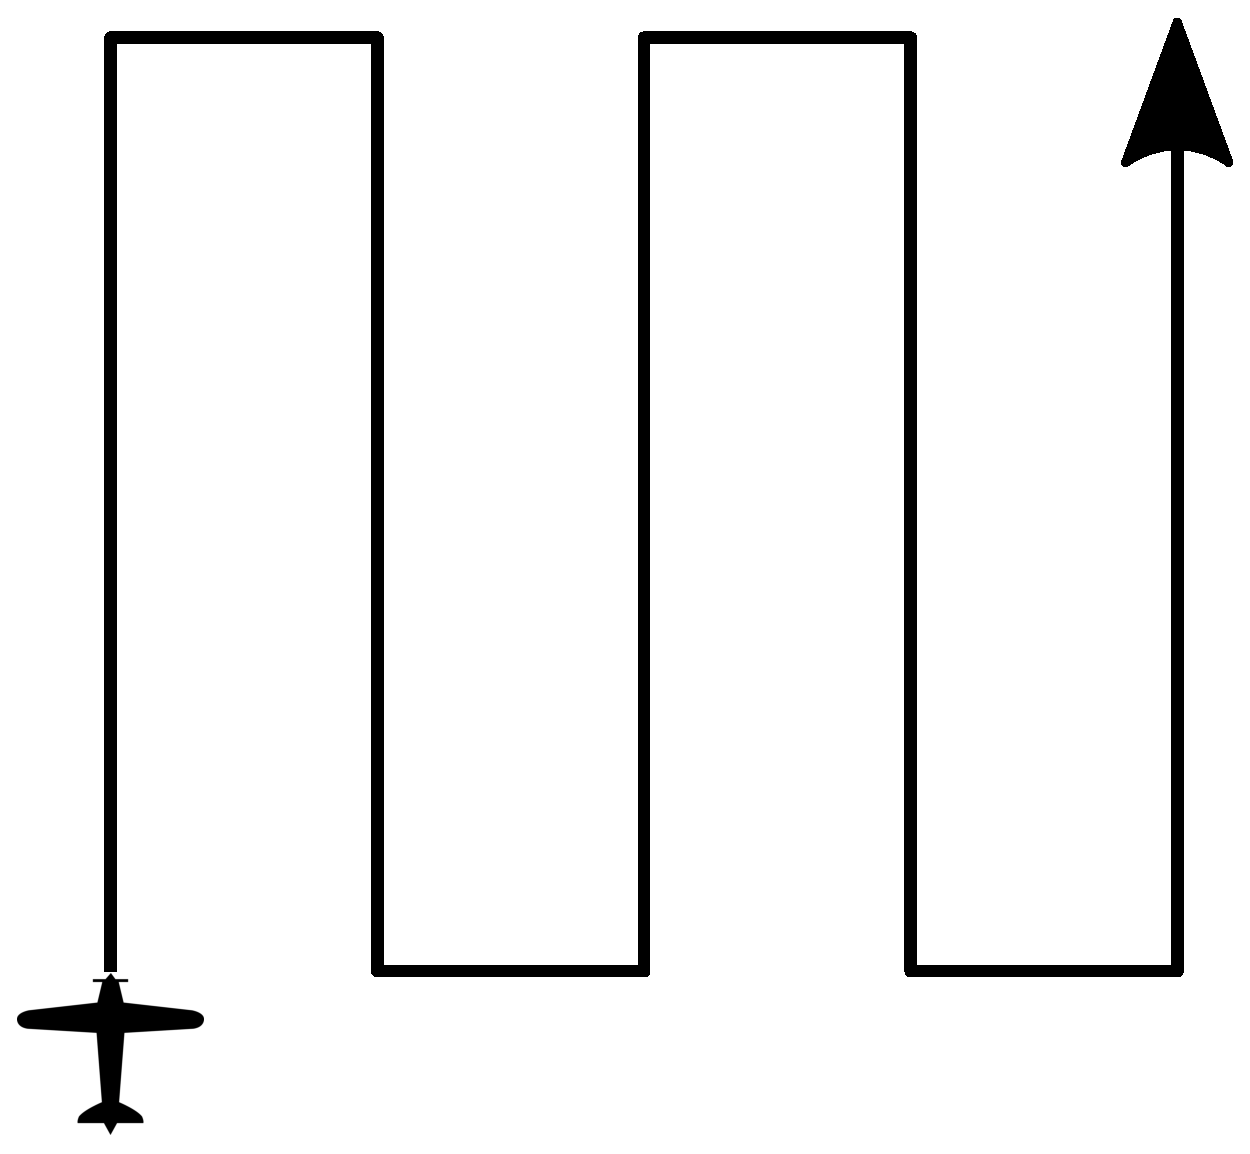
\includegraphics[width=1.0\textwidth]{SimpleLawnmower}
\caption[Simple Lawnmower]{This is the general form of a lawnmower pattern aerial imaging run} %TODO
\label{fig:simplelawnmower}
\end{figure}


%******************************************************************************************************
%******************************************************************************************************
\section{ArduPilot and ArduPlane} 
\label{intro:arduplane}

ArduPilot is an open-source suite of autopilot products aimed at hobbyists and professionals alike 

\subsection{JSBSim}
\label{intro:jsbsim}

JSBSim is the simulator packaged with ArduPlane for testing purposes

%******************************************************************************************************
%******************************************************************************************************
\section{Autopilot Hardware} 
\label{intro:hardware}




%*******************************************************************************
%****************************** Second Chapter *********************************
%*******************************************************************************

\chapter{My second chapter}

\ifpdf
    \graphicspath{{Chapter2/Figs/Raster/}{Chapter2/Figs/PDF/}{Chapter2/Figs/}}
\else
    \graphicspath{{Chapter2/Figs/Vector/}{Chapter2/Figs/}}
\fi


\section[Short title]{Reasonably long section title}

% Uncomment this line, when you have siunitx package loaded.
%The SI Units for dynamic viscosity is \si{\newton\second\per\metre\squared}.
I'm going to randomly include a picture Figure~\ref{fig:minion}.


If you have trouble viewing this document contact Krishna at: \href{mailto:kks32@cam.ac.uk}{kks32@cam.ac.uk} or raise an issue at \url{https://github.com/kks32/phd-thesis-template/}


\begin{figure}[htbp!] 
\centering    

\includegraphics[width=1.0\textwidth]{minion}
\caption[Minion]{This is just a long figure caption for the minion in Despicable Me from Pixar}
\label{fig:minion}
\end{figure}


\section*{Enumeration}
\begin{enumerate}
\item The first topic is dull
\item The second topic is duller
\begin{enumerate}
\item The first subtopic is silly
\item The second subtopic is stupid
\end{enumerate}
\item The third topic is the dullest
\end{enumerate}

\section*{itemize}
\begin{itemize}
\item The first topic is dull
\item The second topic is duller
\begin{itemize}
\item The first subtopic is silly
\item The second subtopic is stupid
\end{itemize}
\item The third topic is the dullest
\end{itemize}

\section*{description}
\begin{description}
\item[The first topic] is dull
\item[The second topic] is duller
\begin{description}
\item[The first subtopic] is silly
\item[The second subtopic] is stupid
\end{description}
\item[The third topic] is the dullest
\end{description}


\clearpage

\tochide\section{Hidden section}
\textbf{Lorem ipsum dolor sit amet}, \textit{consectetur adipiscing elit}. In magna nisi, aliquam id blandit id, congue ac est. Fusce porta consequat leo. Proin feugiat at felis vel consectetur. Ut tempus ipsum sit amet congue posuere. Nulla varius rutrum quam. Donec sed purus luctus, faucibus velit id, ultrices sapien. Cras diam purus, tincidunt eget tristique ut, egestas quis nulla. Curabitur vel iaculis lectus. Nunc nulla urna, ultrices et eleifend in, accumsan ut erat. In ut ante leo. Aenean a lacinia nisl, sit amet ullamcorper dolor. Maecenas blandit, tortor ut scelerisque congue, velit diam volutpat metus, sed vestibulum eros justo ut nulla. Etiam nec ipsum non enim luctus porta in in massa. Cras arcu urna, malesuada ut tellus ut, pellentesque mollis risus.Morbi vel tortor imperdiet arcu auctor mattis sit amet eu nisi. Nulla gravida urna vel nisl egestas varius. Aliquam posuere ante quis malesuada dignissim. Mauris ultrices tristique eros, a dignissim nisl iaculis nec. Praesent dapibus tincidunt mauris nec tempor. Curabitur et consequat nisi. Quisque viverra egestas risus, ut sodales enim blandit at. Mauris quis odio nulla. Cras euismod turpis magna, in facilisis diam congue non. Mauris faucibus nisl a orci dictum, et tempus mi cursus.

Etiam elementum tristique lacus, sit amet eleifend nibh eleifend sed \footnote{My footnote goes blah blah blah! \dots}. Maecenas dapibu augue ut urna malesuada, non tempor nibh mollis. Donec sed sem sollicitudin, convallis velit aliquam, tincidunt diam. In eu venenatis lorem. Aliquam non augue porttitor tellus faucibus porta et nec ante. Proin sodales, libero vitae commodo sodales, dolor nisi cursus magna, non tincidunt ipsum nibh eget purus. Nam rutrum tincidunt arcu, tincidunt vulputate mi sagittis id. Proin et nisi nec orci tincidunt auctor et porta elit. Praesent eu dolor ac magna cursus euismod. Integer non dictum nunc.


\begin{landscape}

\section*{Subplots}
I can cite Wall-E (see Fig.~\ref{fig:WallE}) and Minions in despicable me (Fig.~\ref{fig:Minnion}) or I can cite the whole figure as Fig.~\ref{fig:animations}


\begin{figure}
  \centering
  \begin{subfigure}[b]{0.3\textwidth}
    
\includegraphics[width=\textwidth]{TomandJerry}
    \caption{Tom and Jerry}
    \label{fig:TomJerry}   
  \end{subfigure}             
  \begin{subfigure}[b]{0.3\textwidth}
    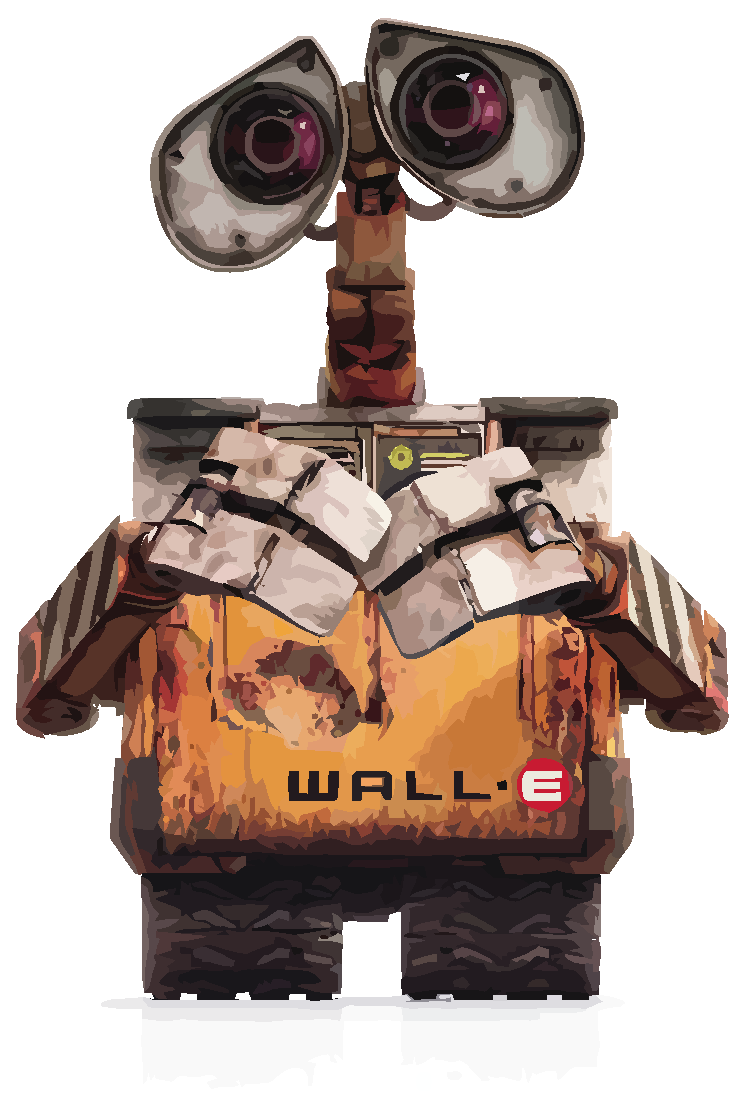
\includegraphics[width=\textwidth]{WallE}
    \caption{Wall-E}
    \label{fig:WallE}
  \end{subfigure}             
  \begin{subfigure}[b]{0.3\textwidth}
    
\includegraphics[width=\textwidth]{minion}
    \caption{Minions}
    \label{fig:Minnion}
  \end{subfigure}
  \caption{Best Animations}
  \label{fig:animations}
\end{figure}


\end{landscape}

\chapter{My third chapter}

% **************************** Define Graphics Path **************************
\ifpdf
    \graphicspath{{Chapter3/Figs/Raster/}{Chapter3/Figs/PDF/}{Chapter3/Figs/}}
\else
    \graphicspath{{Chapter3/Figs/Vector/}{Chapter3/Figs/}}
\fi

\section{First section of the third chapter}
And now I begin my third chapter here \dots

And now to cite some more people~\citet{Rea85,Ancey1996}

\subsection{First subsection in the first section}
\dots and some more 

\subsection{Second subsection in the first section}
\dots and some more \dots

\subsubsection{First subsub section in the second subsection}
\dots and some more in the first subsub section otherwise it all looks the same
doesn't it? well we can add some text to it \dots

\subsection{Third subsection in the first section}
\dots and some more \dots

\subsubsection{First subsub section in the third subsection}
\dots and some more in the first subsub section otherwise it all looks the same
doesn't it? well we can add some text to it and some more and some more and
some more and some more and some more and some more and some more \dots

\subsubsection{Second subsub section in the third subsection}
\dots and some more in the first subsub section otherwise it all looks the same
doesn't it? well we can add some text to it \dots

\section{Second section of the third chapter}
and here I write more \dots

\section{The layout of formal tables}
This section has been modified from ``Publication quality tables in \LaTeX*''
 by Simon Fear.

The layout of a table has been established over centuries of experience and 
should only be altered in extraordinary circumstances. 

When formatting a table, remember two simple guidelines at all times:

\begin{enumerate}
  \item Never, ever use vertical rules (lines).
  \item Never use double rules.
\end{enumerate}

These guidelines may seem extreme but I have
never found a good argument in favour of breaking them. For
example, if you feel that the information in the left half of
a table is so different from that on the right that it needs
to be separated by a vertical line, then you should use two
tables instead. Not everyone follows the second guideline:

There are three further guidelines worth mentioning here as they
are generally not known outside the circle of professional
typesetters and subeditors:

\begin{enumerate}\setcounter{enumi}{2}
  \item Put the units in the column heading (not in the body of
          the table).
  \item Always precede a decimal point by a digit; thus 0.1
      {\em not} just .1.
  \item Do not use `ditto' signs or any other such convention to
      repeat a previous value. In many circumstances a blank
      will serve just as well. If it won't, then repeat the value.
\end{enumerate}

A frequently seen mistake is to use `\textbackslash begin\{center\}' \dots `\textbackslash end\{center\}' inside a figure or table environment. This center environment can cause additional vertical space. If you want to avoid that just use `\textbackslash centering'


\begin{table}
\caption{A badly formatted table}
\centering
\label{table:bad_table}
\begin{tabular}{|l|c|c|c|c|}
\hline 
& \multicolumn{2}{c}{Species I} & \multicolumn{2}{c|}{Species II} \\ 
\hline
Dental measurement  & mean & SD  & mean & SD  \\ \hline 
\hline
I1MD & 6.23 & 0.91 & 5.2  & 0.7  \\
\hline 
I1LL & 7.48 & 0.56 & 8.7  & 0.71 \\
\hline 
I2MD & 3.99 & 0.63 & 4.22 & 0.54 \\
\hline 
I2LL & 6.81 & 0.02 & 6.66 & 0.01 \\
\hline 
CMD & 13.47 & 0.09 & 10.55 & 0.05 \\
\hline 
CBL & 11.88 & 0.05 & 13.11 & 0.04\\ 
\hline 
\end{tabular}
\end{table}

\begin{table}
\caption{A nice looking table}
\centering
\label{table:nice_table}
\begin{tabular}{l c c c c}
\hline 
\multirow{2}{*}{Dental measurement} & \multicolumn{2}{c}{Species I} & \multicolumn{2}{c}{Species II} \\ 
\cline{2-5}
  & mean & SD  & mean & SD  \\ 
\hline
I1MD & 6.23 & 0.91 & 5.2  & 0.7  \\

I1LL & 7.48 & 0.56 & 8.7  & 0.71 \\

I2MD & 3.99 & 0.63 & 4.22 & 0.54 \\

I2LL & 6.81 & 0.02 & 6.66 & 0.01 \\

CMD & 13.47 & 0.09 & 10.55 & 0.05 \\

CBL & 11.88 & 0.05 & 13.11 & 0.04\\ 
\hline 
\end{tabular}
\end{table}


\begin{table}
\caption{Even better looking table using booktabs}
\centering
\label{table:good_table}
\begin{tabular}{l c c c c}
\toprule
\multirow{2}{*}{Dental measurement} & \multicolumn{2}{c}{Species I} & \multicolumn{2}{c}{Species II} \\ 
\cmidrule{2-5}
  & mean & SD  & mean & SD  \\ 
\midrule
I1MD & 6.23 & 0.91 & 5.2  & 0.7  \\

I1LL & 7.48 & 0.56 & 8.7  & 0.71 \\

I2MD & 3.99 & 0.63 & 4.22 & 0.54 \\

I2LL & 6.81 & 0.02 & 6.66 & 0.01 \\

CMD & 13.47 & 0.09 & 10.55 & 0.05 \\

CBL & 11.88 & 0.05 & 13.11 & 0.04\\ 
\bottomrule
\end{tabular}
\end{table}

%%******************************************************************************************************
%******************************* Fourth Chapter *******************************************************
%******************************************************************************************************
\chapter{Task Two: Path Following}
\label{task2}

% **************************** Define Graphics Path **************************
\ifpdf
    \graphicspath{{Chapter4/Figs/Raster/}{Chapter4/Figs/PDF/}{Chapter4/Figs/}}
\else
    \graphicspath{{Chapter4/Figs/Vector/}{Chapter4/Figs/}}
\fi

%******************************************************************************************************
%******************************************************************************************************
\section{The Problem}
\label{task2:description}


%******************************************************************************************************
%******************************************************************************************************
\section{Solution}
\label{task2:solution}
%%******************************** Fifth Chapter *******************************************************
%******************************************************************************************************
\chapter{Future Work}
\label{future}

% **************************** Define Graphics Path **************************
\ifpdf
    \graphicspath{{Chapter5/Figs/Raster/}{Chapter5/Figs/PDF/}{Chapter5/Figs/}}
\else
    \graphicspath{{Chapter5/Figs/Vector/}{Chapter5/Figs/}}
\fi

%******************************************************************************************************
%******************************************************************************************************
\section{Proposal 1: Incorporation into MissionPlanner}
\label{future:missionplanner}
%%******************************** Sixth Chapter *******************************************************
%******************************************************************************************************
\chapter{Project Planning and Management}
\label{planning}

% **************************** Define Graphics Path **************************
\ifpdf
    \graphicspath{{Chapter6/Figs/Raster/}{Chapter6/Figs/PDF/}{Chapter6/Figs/}}
\else
    \graphicspath{{Chapter6/Figs/Vector/}{Chapter6/Figs/}}
\fi

%******************************************************************************************************
%******************************************************************************************************
\section{Agile Planning}
\label{planning:agile}
%%******************************** Seventh Chapter *****************************************************
%******************************************************************************************************
\chapter{Summary and Conclusions}
\label{conclusion}

% **************************** Define Graphics Path **************************
\ifpdf
    \graphicspath{{Chapter7/Figs/Raster/}{Chapter7/Figs/PDF/}{Chapter7/Figs/}}
\else
    \graphicspath{{Chapter7/Figs/Vector/}{Chapter7/Figs/}}
\fi

%******************************************************************************************************
%******************************************************************************************************
\section{Conclusions}
\label{conclusion:conclusion}



% ********************************** Back Matter *******************************
% Backmatter should be commented out, if you are using appendices after References
%\backmatter

% ********************************** Bibliography ******************************
\begin{spacing}{0.9}

% To use the conventional natbib style referencing
% Bibliography style previews: http://nodonn.tipido.net/bibstyle.php
% Reference styles: http://sites.stat.psu.edu/~surajit/present/bib.htm

\bibliographystyle{apalike}
%\bibliographystyle{plainnat} % use this to have URLs listed in References
\cleardoublepage
\bibliography{References/references} % Path to your References.bib file


% If you would like to use BibLaTeX for your references, pass `custombib' as
% an option in the document class. The location of 'reference.bib' should be
% specified in the preamble.tex file in the custombib section.
% Comment out the lines related to natbib above and uncomment the following line.

%\printbibliography[heading=bibintoc, title={References}]


\end{spacing}

% ********************************** Appendices ********************************

\begin{appendices} % Using appendices environment for more functunality

% ******************************* Thesis Appendix A ********************************
\chapter{How to install \LaTeX} 

\section*{Windows OS}

\subsection*{TeXLive package - full version}
\begin{enumerate}
\item	Download the TeXLive ISO (2.2GB) from\\
\href{https://www.tug.org/texlive/}{https://www.tug.org/texlive/}
\item	Download WinCDEmu (if you don't have a virtual drive) from \\
\href{http://wincdemu.sysprogs.org/download/}{http://wincdemu.sysprogs.org/download/}
\item	To install Windows CD Emulator follow the instructions at\\
\href{http://wincdemu.sysprogs.org/tutorials/install/}{http://wincdemu.sysprogs.org/tutorials/install/}
\item	Right click the iso and mount it using the WinCDEmu as shown in \\
\href{http://wincdemu.sysprogs.org/tutorials/mount/}{http://wincdemu.sysprogs.org/tutorials/mount/}
\item	Open your virtual drive and run setup.pl
\end{enumerate}

or

\subsection*{Basic MikTeX - TeX distribution}
\begin{enumerate}
\item	Download Basic-MiK\TeX (32bit or 64bit) from\\
\href{http://miktex.org/download}{http://miktex.org/download}
\item	Run the installer 
\item	To add a new package go to Start >> All Programs >> MikTex >> Maintenance (Admin) and choose Package Manager
\item	Select or search for packages to install
\end{enumerate}

\subsection*{TexStudio - Tex Editor}
\begin{enumerate}
\item	Download TexStudio from\\
\href{http://texstudio.sourceforge.net/\#downloads}{http://texstudio.sourceforge.net/\#downloads} 
\item	Run the installer
\end{enumerate}

\section*{Mac OS X}
\subsection*{MacTeX - TeX distribution}
\begin{enumerate}
\item	Download the file from\\
\href{https://www.tug.org/mactex/}{https://www.tug.org/mactex/}
\item	Extract and double click to run the installer. It does the entire configuration, sit back and relax.
\end{enumerate}

\subsection*{TexStudio - Tex Editor}
\begin{enumerate}
\item	Download TexStudio from\\
\href{http://texstudio.sourceforge.net/\#downloads}{http://texstudio.sourceforge.net/\#downloads} 
\item	Extract and Start
\end{enumerate}


\section*{Unix/Linux}
\subsection*{TeXLive - TeX distribution}
\subsubsection*{Getting the distribution:}
\begin{enumerate}
\item	TexLive can be downloaded from\\
\href{http://www.tug.org/texlive/acquire-netinstall.html}{http://www.tug.org/texlive/acquire-netinstall.html}.
\item	TexLive is provided by most operating system you can use (rpm,apt-get or yum) to get TexLive distributions
\end{enumerate}

\subsubsection*{Installation}
\begin{enumerate}
\item	Mount the ISO file in the mnt directory
\begin{verbatim}
mount -t iso9660 -o ro,loop,noauto /your/texlive####.iso /mnt
\end{verbatim}

\item	Install wget on your OS (use rpm, apt-get or yum install)
\item	Run the installer script install-tl.
\begin{verbatim}
	cd /your/download/directory
	./install-tl
\end{verbatim}
\item	Enter command `i' for installation

\item	Post-Installation configuration:\\
\href{http://www.tug.org/texlive/doc/texlive-en/texlive-en.html\#x1-320003.4.1}{http://www.tug.org/texlive/doc/texlive-en/texlive-en.html\#x1-320003.4.1} 
\item	Set the path for the directory of TexLive binaries in your .bashrc file
\end{enumerate}

\subsubsection*{For 32Bit OS}
For Bourne-compatible shells such as bash, and using Intel x86 GNU/Linux and a default directory setup as an example, the file to edit might be \begin{verbatim}
edit $~/.bashrc file and add following lines
PATH=/usr/local/texlive/2011/bin/i386-linux:$PATH; 
export PATH 
MANPATH=/usr/local/texlive/2011/texmf/doc/man:$MANPATH;
export MANPATH 
INFOPATH=/usr/local/texlive/2011/texmf/doc/info:$INFOPATH;
export INFOPATH
\end{verbatim}
\subsubsection*{For 64Bit}
\begin{verbatim}
edit $~/.bashrc file and add following lines
PATH=/usr/local/texlive/2011/bin/x86_64-linux:$PATH;
export PATH 
MANPATH=/usr/local/texlive/2011/texmf/doc/man:$MANPATH;
export MANPATH 
INFOPATH=/usr/local/texlive/2011/texmf/doc/info:$INFOPATH;
export INFOPATH

\end{verbatim}



%\subsection{Installing directly using Linux packages} 
\subsubsection*{Fedora/RedHat/CENTOS:}
\begin{verbatim} 
sudo yum install texlive 
sudo yum install psutils 
\end{verbatim}


\subsubsection*{SUSE:}
\begin{verbatim}
sudo zypper install texlive
\end{verbatim}


\subsubsection*{Debian/Ubuntu:}
\begin{verbatim} 
sudo apt-get install texlive texlive-latex-extra 
sudo apt-get install psutils
\end{verbatim}

% ******************************* Thesis Appendix B ********************************

\chapter{Installing the CUED Class file}

\LaTeX.cls files can be accessed system-wide when they are placed in the
<texmf>/tex/latex directory, where <texmf> is the root directory of the user’s \TeX installation. On systems that have a local texmf tree (<texmflocal>), which
may be named ``texmf-local'' or ``localtexmf'', it may be advisable to install packages in <texmflocal>, rather than <texmf> as the contents of the former, unlike that of the latter, are preserved after the \LaTeX system is reinstalled and/or upgraded.

It is recommended that the user create a subdirectory <texmf>/tex/latex/CUED for all CUED related \LaTeX class and package files. On some \LaTeX systems, the directory look-up tables will need to be refreshed after making additions or deletions to the system files. For \TeX Live systems this is accomplished via executing ``texhash'' as root. MIK\TeX users can run ``initexmf -u'' to accomplish the same thing.

Users not willing or able to install the files system-wide can install them in their personal directories, but will then have to provide the path (full or relative) in addition to the filename when referring to them in \LaTeX.



\end{appendices}

% *************************************** Index ********************************
\printthesisindex % If index is present

\end{document}
